\documentclass[a4j,12pt,onecolumn,oneside,final]{jreport}

%\usepackage{gthesis}
\usepackage{gthesis_myown}

\usepackage{amsmath,amsthm,amssymb,ascmac}
%\usepackage{fancybox}
\usepackage{slashbox}
\usepackage[dvipdfmx]{graphicx}
\usepackage[dvipdfmx]{color}
%\usepackage[dviout]{color,graphics}
\usepackage{graphicx}
\usepackage{color}
%\usepackage{psfrag}
%\usepackage{upgreek}
\usepackage{bm}
%\usepackage{wrapfig}

%%%%%%%%%%%%%%%%%%%%%%%%%%%%%%%%%%%%%%%%%%%%%%%%%%%%%%%%%%%%%%%%
% put local tex-macros in this file %

%%%%%%%%%%%%%%%%%%%%%%%%%%%%%
%色設定
%%%%%%%%%%%%%%%%%%%%%%%%%%%%%
\definecolor{Black}{rgb}{0.0,0.0,0.0}
\definecolor{Red}{rgb}{0.9,0.0,0.1}
\definecolor{Blue}{rgb}{0.1,0.1,0.5}
\definecolor{Green}{rgb}{0.1,0.4,0.1}
\definecolor{Gray}{rgb}{0.75,0.85,0.9} % Fuji-iro
\definecolor{Shade}{rgb}{0.1,0.1,0.4}

%%%%%%%%%%%%%%%%%%%%%%%%%%%%%%%%%%%%%%%%%%%%%%%%%%%%%%%%%%%%%%%%
\年度{令和元年度}
\提出年月{令和2年1月}

\題名{光沢感知覚に対する色度情報の寄与}
\梗概題名{光沢感知覚に対する色度情報の寄与}

\指導教員名A{永井 岳大}
\職名A{准教授}

\指導教員名B{}
\職名B{}

\所属学科{情報通信系}{}
\学籍番号{16B16967}
\氏名{渡辺 侑真}

\内容梗概{研究の背景と目的はカクカクシカジカ.
研究の背景と目的はカクカクシカジカ.
研究の背景と目的はカクカクシカジカ.
研究の背景と目的はカクカクシカジカ.

従来の研究成果はカクカクシカジカ.
従来の研究成果はカクカクシカジカ.
従来の研究成果はカクカクシカジカ.
従来の研究成果はカクカクシカジカ.

本研究では新たにカクカクシカジカの検討を行なった.
本研究では新たにカクカクシカジカの検討を行なった.
本研究では新たにカクカクシカジカの検討を行なった.
本研究では新たにカクカクシカジカの検討を行なった.

その結果,カクカクシカジカの成果と得ることができた.
その結果,カクカクシカジカの成果と得ることができた.
その結果,カクカクシカジカの成果と得ることができた.
その結果,カクカクシカジカの成果と得ることができた.

従来の成果に比べて本研究で得られた成果は大変優れている.
従来の成果に比べて本研究で得られた成果は大変優れている.
従来の成果に比べて本研究で得られた成果は大変優れている.
従来の成果に比べて本研究で得られた成果は大変優れている.

残された課題としてはチョメチョメが挙げられる.
残された課題としてはチョメチョメが挙げられる.
}


\begin{document}
% ----------------------------------------------------------------------
% 表紙
\maketitle
% ----------------------------------------------------------------------
% 目次
\setcounter{page}{1}
\renewcommand{\thepage}{\roman{page}}
\setcounter{tocdepth}{1}
\tableofcontents
\clearpage
% ----------------------------------------------------------------------
% 内容
\setcounter{page}{1}
\renewcommand{\thepage}{\arabic{page}}
%\chapter{Introduction}
\chapter{序論}
    \section{研究背景}

    ヒトは物体を見た時に, 瞬時にその質感を把握することができる.
    網膜像を生み出す物理的要因として,照明環境,物体の光学特性,物体の三次元形状があるが,それらは強くかつ複雑に相互作用する.
    この中で,質感とは主に物体の光学特性に対応する知覚であると考えることができる.
    この枠組みで考えれば,網膜像から質感を推定する問題はいわゆる不良設定問題であるにも関わらず,ヒトが容易に質感を知覚できることから,その仕組みを明らかにするための研究がここ15年ほど活発に行われてきた.

    質感の種類は非常に多種多様であるが\cite{Material},その質感の中でも,光沢感を知覚する際の視覚系の情報処理の仕組みについては多く研究されてきた.
    光沢感とは,物体の表面の光学的反射特性に対応する心理的な属性である.
    例えば,パチンコ玉のように表面が非常に平滑な平面においては,鏡面反射が支配的であり,周辺環境の明瞭な像が映り込むことにより非常に強い光沢感が知覚される.
    一方で布のように表面に凹凸が多く存在する平面においては,拡散反射が支配的であり,光沢感はほとんど知覚されない.

    光沢感については,多くの場合その輝度条件と光沢感知覚の関連性について多くの報告がなされてきた.[todo: 先行研究を引用]

    例えば, 物体における鏡面反射成分の面積・コントラスト・シャープネスが光沢知覚に寄与することが先行研究によって明らかとなっている.


    
    しかし,輝度と知覚的な明るさは必ずしも一致するとは限らない.
    例えば,刺激の輝度は同一でも,Helmholtz-Kohlrausch効果による明るさの増幅は色相によって異なることが知られている.
    では,光沢知覚には輝度と明るさ感のうちどちらが寄与しているのだろうか.
    また,Nishidaら(2010)はハイライトの色をつけすぎるとハイライトがハイライトに見えなくなり,それに伴い光沢感が大幅に減衰することを報告した.\cite{Nishida}
    しかし,それは極端に不自然な例であり,日常の光沢感知覚に対する色情報の寄与に関する研究ではない.


    \section{本研究の目的}
    \section{本論文の構成}
%\chapter{Preliminaries}
\chapter{実験1}

\section{目的}

    実験1では,輝度は同一であるが色度のみが異なる刺激に対して知覚される光沢感を測定する.
    色度ごとの光沢感を定量化することで,光沢感に色度情報が寄与しているかどうかを明らかにすることを目的とする.

    \subsection{仮説}

        第1章で述べたとおり,物体の表面の輝度成分が光沢感知覚に寄与していることは既知である.
        しかし,輝度が変わると当然知覚的な明るさも変わるため,光沢感に寄与しているのが知覚的な明るさ感なのか輝度情報そのものなのかについては明らかになっていない.
        輝度と知覚的な明るさ感が分離される現象としてHelmholtz-Kohlrausch効果(以下H-K効果)が知られている.
        これは,同一の輝度を有する色でも彩度が高いほど明るく感じられ,特に青・紫・赤紫・赤などの色相を有する色がより明るく見えるという効果である.
        このように,有彩色刺激を採用しH-K効果を利用することにより,輝度の明るさを分離することが可能となる.

        本研究で検証する仮説は,拡散反射成分と鏡面反射成分の知覚的な明るさ感のコントラストが主に光沢感に寄与しているというものである.
        従来の研究から,拡散反射成分と鏡面反射成分の輝度コントラストが知覚的光沢感に強く寄与することが明らかになっている.[参考文献]
        本実験で検証するのは,この輝度コントラストに起因するものであったという可能性に関する仮説となる.ここで,鏡面反射成分と拡散反射成分の色度情報を利用して明るさ感のみを変化させれば,輝度の効果と明るさの効果を検証できるはずである.
        反射成分のうち,拡散反射成分は鏡面反射成分に比べて多くの場合には低輝度である.
        そこで反射成分を拡散反射成分と鏡面反射成分に分け,拡散反射成分のみに輝度を変えずに色度を変化させ有彩色を付与する処理を行う.
        このとき,もし上述の仮説が正しいとすれば,H-K効果による明るさ感の増幅が顕著な色度では,拡散反射成分の明るさ感がH-K効果により向上することに起因し,他色度に比べて相対的に明るさ感のコントラストが大きく減少するため,光沢感が小さくなるはずである.
        すなわち,H-K効果の明るさの増幅度合いと光沢感には負の相関が現れる.

\section{実験方法}
    \subsection{被験者}
        本実験は20代男性7人に対して行われた.
        全被験者の視力または矯正視力は正常であり,かつ石原式色覚異常検査表により色覚が正常であることが確認されていた.

    \subsection{実験環境}

        \begin{figure}[h]
            \centering
            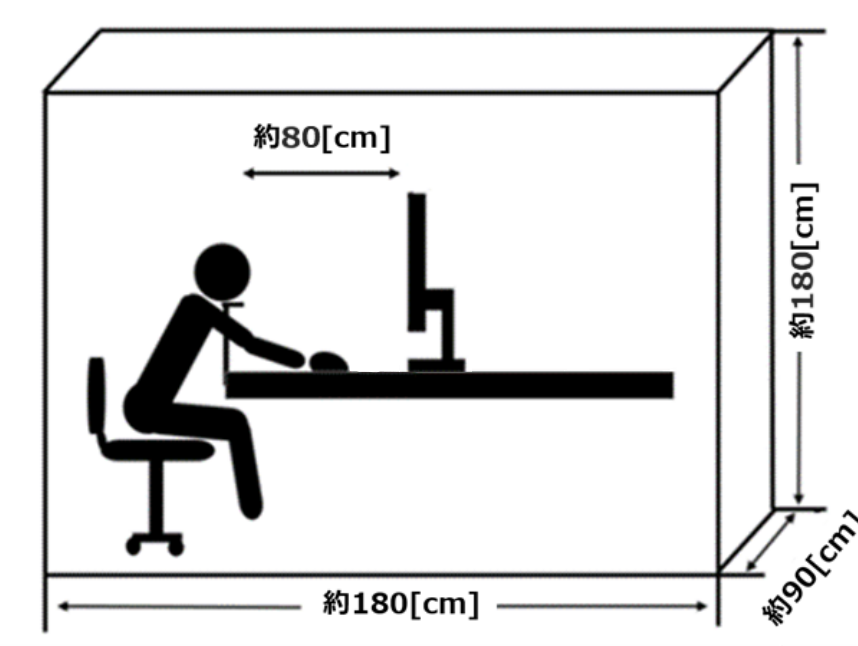
\includegraphics[width=10.0cm]{./img/darkroom_p.png}
            \caption{実験環境概略図}
            \label{darkroom}
        \end{figure}

        図\ref{darkroom}に実験環境の概略図を示す.
        暗幕で覆われた簡易的な暗室内に刺激呈示用液晶ディスプレイ (EIZO社, 解像度 1920 ピクセル✕ 1200 ピクセル, リフレッシュレート 60 Hz) を設置し実験を行った.
        また,刺激の輝度と色度を正確に投影するために分光反射輝度計 (Cambridge Research Systems 社 SpectroCAL) によりモニタの分光分布を,色彩輝度計 (Cambridge Research Systems 社 ColorCAL2) によりモニタのガンマ特性を測定した.
        これにより,所望のCIE $XYZ$三刺激値をモニタに呈示することが可能となった.
        
        実験はすべてPC ( DELL 社 Vostro 13 5000, OS: Ubuntu 18.04.3 LTS) で統制され,MathWorks MATLAB と Psychtoolbox3\cite{Psychtoolbox} を用いてプログラムを作成・実行することでディスプレイの刺激呈示と被験者応答を管理した.
        実験中,被験者の頭部はディスプレイから 80 cm の距離に顎台により固定され,両眼自然視でディスプレイを観察した.
        被験者はトラックボールマウスを使用して応答した.

    \subsection{実験刺激}

        \begin{figure}[h]
            \centering
            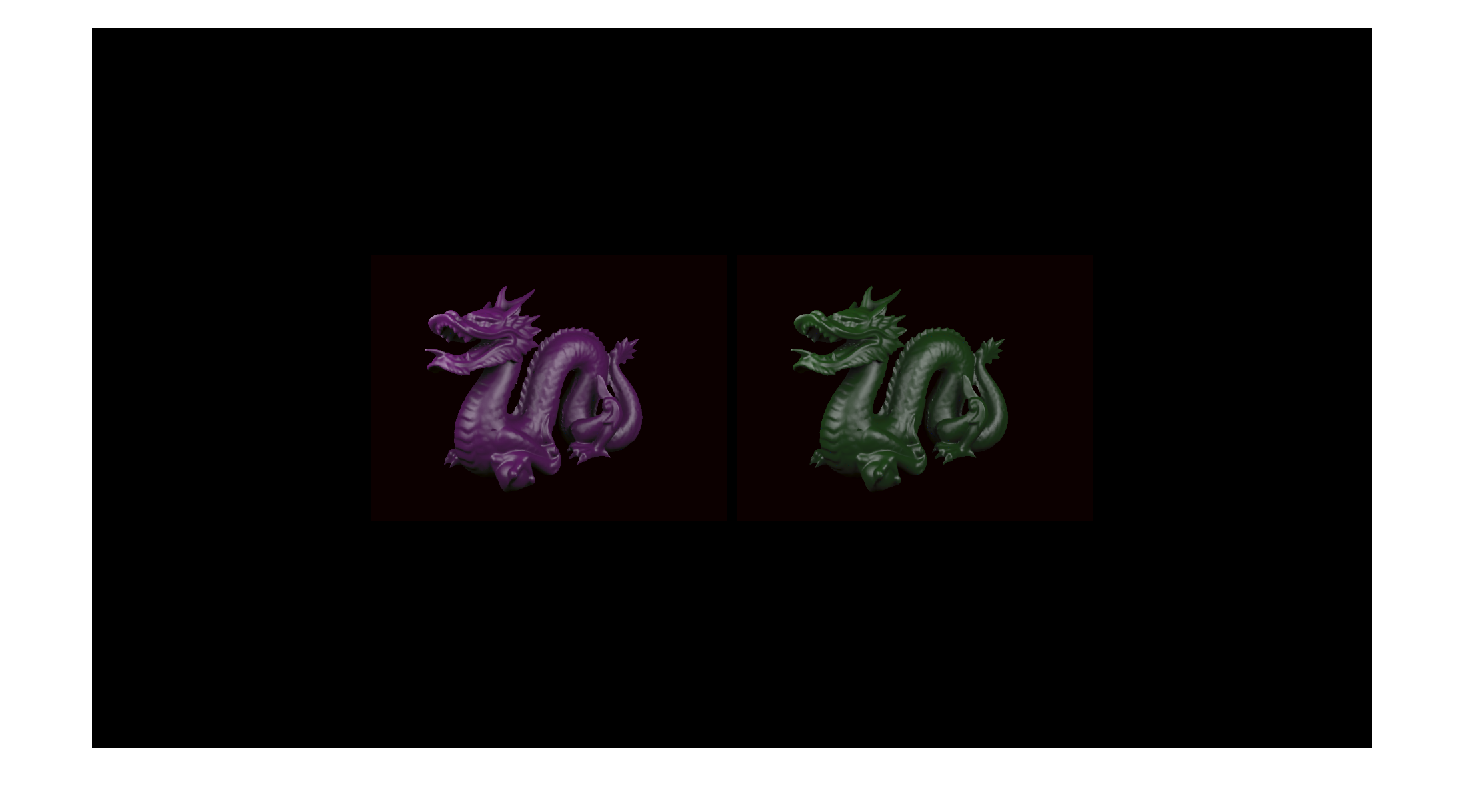
\includegraphics[width=14.0cm]{./img/ex1_stimuli.png}
            \caption{実験刺激の例}
            \label{ex1_stimuli}
        \end{figure}

        図\ref{ex1_stimuli}に実験1で使用する刺激を示す.
        刺激は黒背景上の中心部分の縦 6.42 deg, 横 17.35 deg の範囲の左右に呈示される二枚のコンピュータグラフィックス画像であった.
        これらの画像はモニタ中央を挟んで対称な位置に呈示された.
        また,各画像はコンピュータグラフィックスソフトウェアを用いたレンダリングと,MATLAB上での簡易的な画像処理を用いた着色の二つの工程を経て作られた.
        以下に,これらの工程の詳細を記す.

        \subsubsection{レンダリング}

            実験に用いた刺激の元となる無彩色刺激は RenderToolbox4 によって, レンダラーを Mitsuba\cite{Mitsuba} として作成された.
            この際の照明環境はCIE標準光源D65であり,物体の分光反射特性は全波長にわたり同じ値であった.
            物体形状として,Stanford Dragon と Stanford Bunny \cite{StanfordModels} の2種類を使用し,照明環境も含めた環境のジオメトリはBlender 2.79により設定した.
            一方,表面反射特性は RenderToolbox4 と Mitsuba により設定し,その反射モデルとして Ward モデル\cite{Ward}を用いた.
            この際,拡散反射成分と鏡面反射成分の色度を別々に操作するため,これらの反射成分は独立にレンダリングした.
            このレンダリングにおけるパラメータを表\ref{render_param}に示す.

            \begin{table}[h]
                \centering
                \caption{レンダリング時のパラメータ}
                \begin{tabular}{|l||c|c|c|} \hline
                                           & SpecularReflectance & DiffuseReflectance & Roughness \\ \hline \hline
                    拡散反射成分           & 0                   & 0.1                & 0.2 \\ \hline
                    鏡面反射成分           & 0.9                 & 0                  & 0.2 \\ \hline
                \end{tabular}
                \label{render_param}
            \end{table}
        
        \subsubsection{着色}

            レンダリングされた画像は上述したとおりD65の色度を持つ画像であったが,その画像に対して色条件を設定するために色度を付与した.
            その方法はSD着色とD着色の2種類であった.
            SD着色では,拡散反射成分と鏡面反射成分の両方に同じ色度を設定し,それらのCIE $XYZ$値を加算して作成した.
            D着色では,拡散反射成分にのみ着色を行い,$XYZ$値を加算して作成した.
            この着色処理において,Mitsubaによってレンダリングされた画像のXYZ三刺激値を $u^{\prime}v^{\prime}Y$ 色空間に変換し, $u^{\prime}v^{\prime}$ 色度図上で行われた.
            その色度は全部で9種類である.
            そのうち1種類はD65の色度であり,これを白色点とする.
            その他の8種類の色度は,白色点を中心とし,$u^{\prime}v^{\prime}$ 色度図上の0°から45°間隔となる8方向にある色度であった.
            本論文では,これらの9色度をそれぞれgray, red, orange, yellow, green, blue-green, cyan, blue, magentaと呼ぶことにする.

            レンダリングされた画像は高輝度域を含む画像であった.
            モニタが表示可能な色域は輝度によって異なり,特にモニタが表示できる最大・最小輝度付近における $u^{\prime}v^{\prime}$ 色度図の領域は非常に小さい.
            すなわち,この画像に対して着色処理を行った場合,高輝度になりやすい鏡面反射成分に十分な彩度の色度を付与することができない.
            このため,線形トーンマッピングによって画像の最高輝度を下げた.

            また,モニタが表示可能な色域は色相によっても異なる.レンダリングされた画像にモニタの色域外の色度を付与しないように,画像の輝度を対数尺度を用いて200段階に標本化し,そのそれぞれの輝度に対して9種類の色度の白色点から最大距離となる点を計測した.


    \subsection{実験手続き}

        \begin{figure}[h]
            \centering
            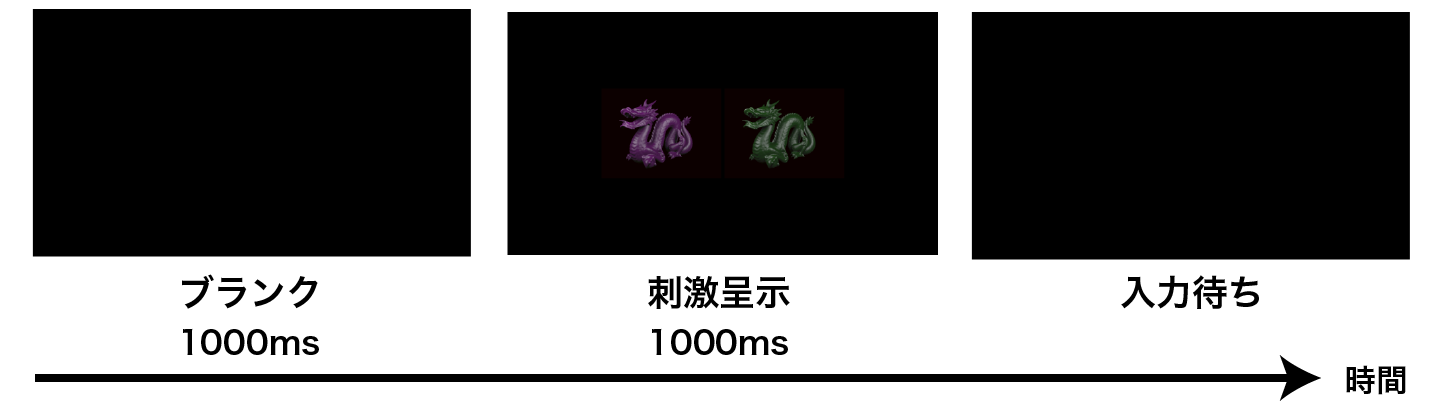
\includegraphics[width=14.0cm]{./img/ex1_procedure.png}
            \caption{1試行の流れ}
            \label{ex1_procedure}
        \end{figure}

        実験1はサーストンの一対比較法を用いて行われた.
        実験1の1試行の流れを図\ref{ex1_procedure}に示す.各試行はまず黒背景のみからなるブランク画面の1000msの呈示から始まる.
        その後,刺激対が1000msの間呈示され,さらに,色順応を避けるために黒背景のみからなる入力待ち画面に移行した.
        刺激対の呈示中または入力待ち画面で,被験者は右画像と左画像のうちどちらからより光沢感を強く知覚するかを,マウスの左クリックまたは右クリックにより応答した.
        このとき次の試行のブランク画面に移行した.

        各セッションは 2 着色条件 $\times$ 物体形状 2 種類 $\times$ 色の組み合わせ 36 通り = 144 試行からなる.
        各被験者は全体で4セッションの実験を行った.
        各セッションの 144 試行で使われる刺激対は全てランダムな順序で選ばれた.
        1セッションに要する時間はおよそ8分であり,2セッション目と3セッション目の間に一度だけ休憩をとった.



\section{実験結果}
    \subsection{解析方法}

    \subsection{考察}
        
        \begin{figure}[h]
            \centering
            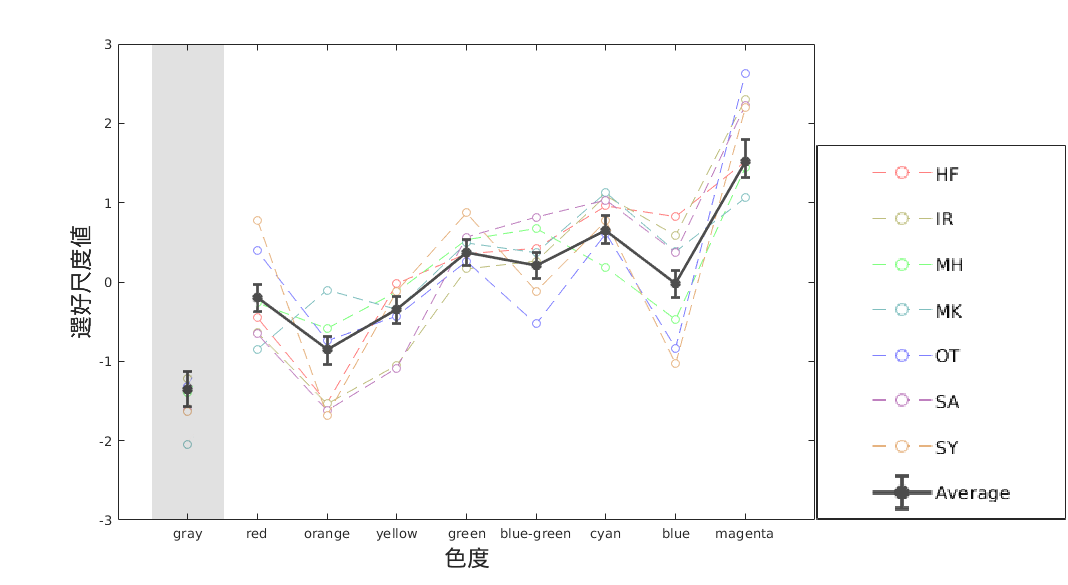
\includegraphics[width=14.0cm]{./img/ex1_res_DSD_p.png}
            \caption{Dragon形状のSD条件における選好尺度値}
            \label{ex1_DSD}
        \end{figure}

        \begin{figure}[h]
            \centering
            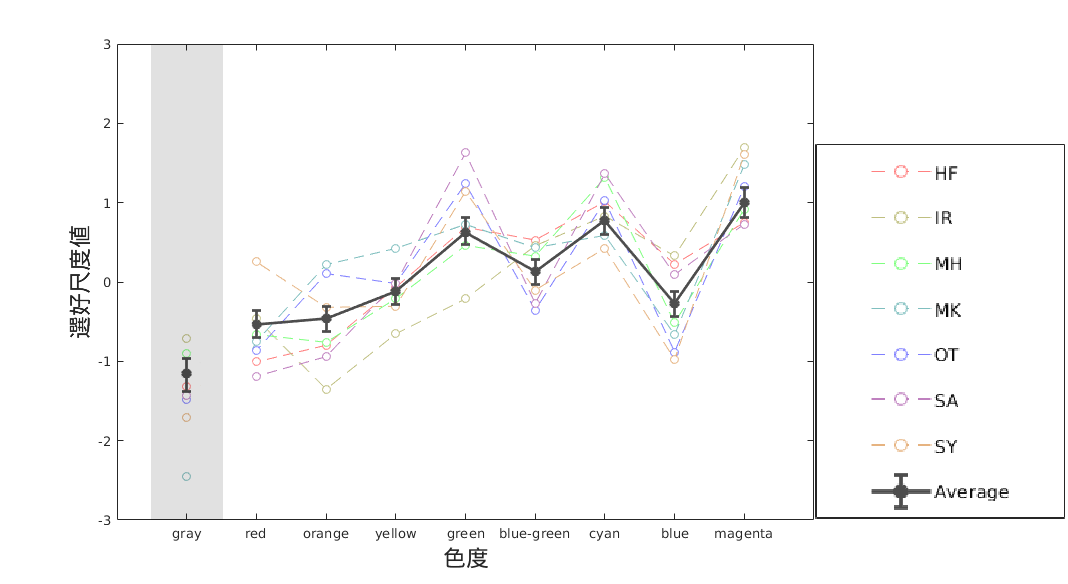
\includegraphics[width=14.0cm]{./img/ex1_res_BSD_p.png}
            \caption{Bunny形状のSD条件における選好尺度値}
            \label{ex1_BSD}
        \end{figure}

        \begin{figure}[h]
            \centering
            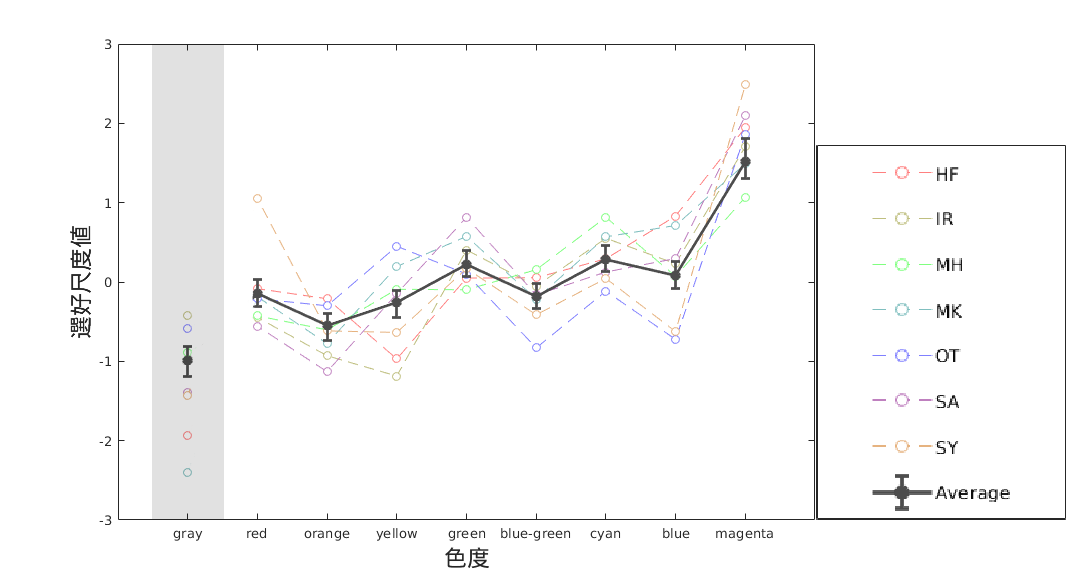
\includegraphics[width=14.0cm]{./img/ex1_res_DD_p.png}
            \caption{Dragon形状のD条件における選好尺度値}
            \label{ex1_DD}
        \end{figure}

        \begin{figure}[h]
            \centering
            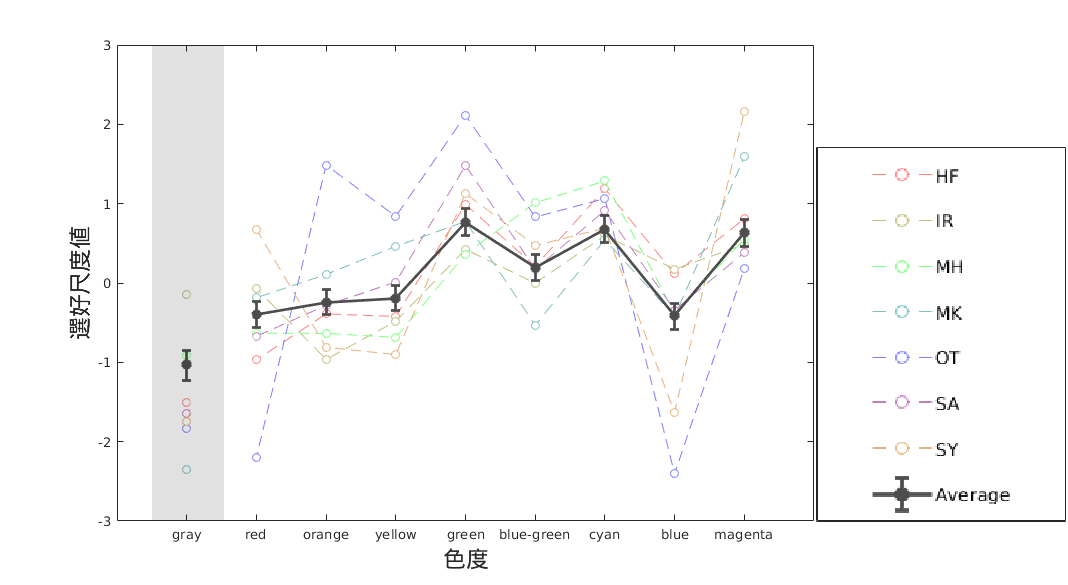
\includegraphics[width=14.0cm]{./img/ex1_res_BD_p.png}
            \caption{Bunny形状のD条件における選好尺度値}
            \label{ex1_BD}
        \end{figure}

        物体形状や着色条件に関わらず,すべての条件において色度により光沢感が異なることがわかる.
        特にBunny形状のD条件を除いてmagentaの光沢感が極めて高く,次いでgreen,cyanの光沢感が高いという結果となった.
        Dragon形状のSD条件, Bunny形状のSD条件, Dragon形状のD条件で似た傾向が見られたが,Bunny形状のD条件ではblueとmagentaの光沢感が相対的に低い値であった.

        仮説通りであれば,D条件においてredやmagentaの色度における光沢感は他の色度に比べて低いはずであるが,Dragon,Bunnyの両方でそのような傾向は見られない.
        このため,光沢感が拡散反射と鏡面反射の知覚的な明るさのコントラストによって主に決まっているという訳ではないと言える.

        ここで,SD着色条件とD着色条件で傾向に大きな違いが見られないこと,magentaの光沢感が極端に大きいことに着目する.
        明るさのコントラストではなく,刺激全体を通して感じられる明るさが光沢感に寄与しているのではないかと考え,次の実験2を行った.

    \subsection{選好尺度値}
\chapter{実験2 -光沢感と明るさ感の関連性-}

    \section{目的}

        実験2では,実験1で使用した刺激と同じ色度を持つ単色パッチを用いて,H-K効果,すなわち色度による明るさ感の変化を用いて明るさを定量化する.
        実験1の色度による光沢感の変化と,実験2で計測される色度による明るさ感の変化を比較することで,色度による明るさ感の変化が光沢感に影響を及ぼした可能性について検討する.


    \section{実験方法}
        \subsection{実験環境,被験者}

            実験2で用いた装置と参加した被験者は,いずれも実験1と同一であった.

        \subsection{実験刺激}

            \begin{figure}[h]
                \centering
                
\includegraphics[width=14.0cm]{./img/ex2_stimuli2.png}
                \caption{実験刺激の例}
                \label{ex2_stimuli}
            \end{figure}

            \begin{figure}[h]
                \centering
                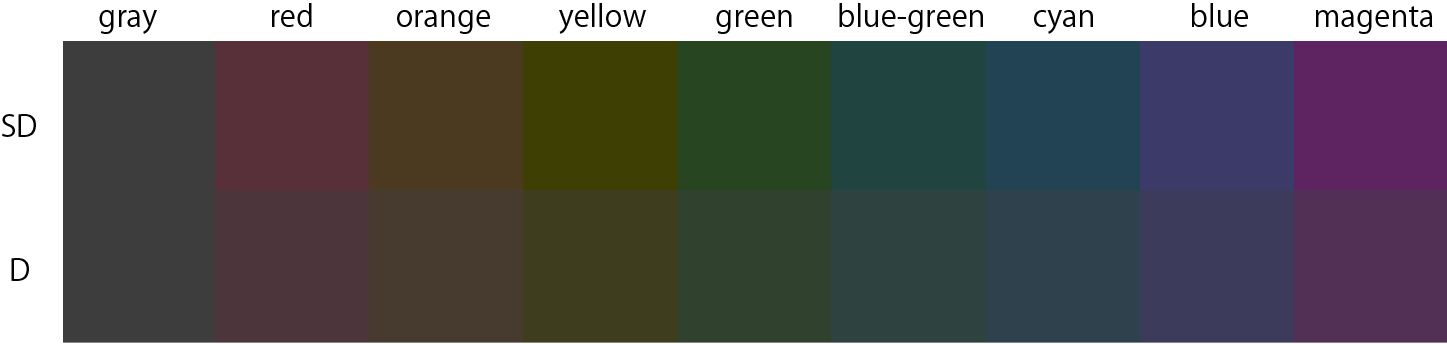
\includegraphics[width=14.0cm]{./img/ex2_stimuli_p.png}
                \caption{参照刺激として使われた色}
                \label{ex2_stimuli_set}
            \end{figure}
            \newpage

            実験2で使用する刺激と,参照刺激に使われた色を図\ref{ex2_stimuli}と図\ref{ex2_stimuli_set}に示す.
            参照刺激として使われた18種類の色度は,実験1で用いたDragon形状におけるSD条件,D条件のそれぞれの刺激の$XYZ$平均色に対応する.
            その輝度は,いずれの色度,彩色条件において5.80${\rm cd/m}^2$であった.

        \subsection{実験手続き}

            \begin{figure}[h]
                \centering
                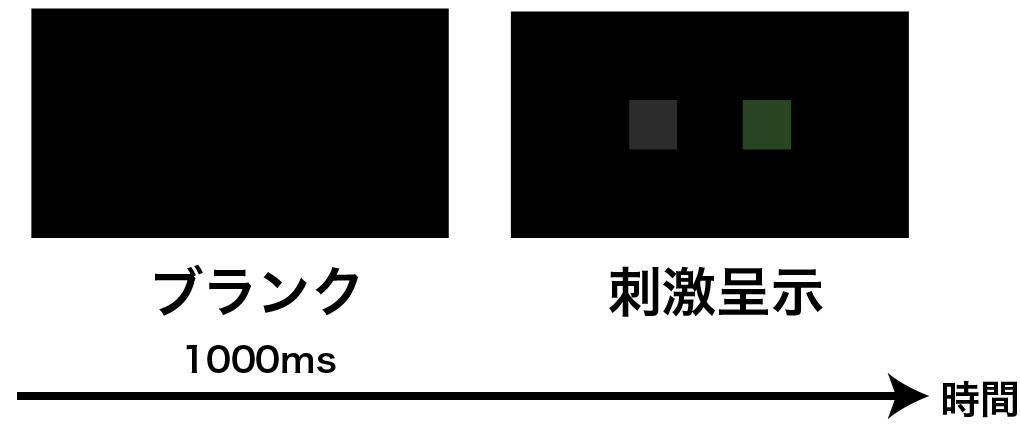
\includegraphics[width=10.0cm]{./img/ex2_procedure.png}
                \caption{1試行の流れ}
                \label{ex2_procedure}
            \end{figure}

            実験2では調整法によりカラーパッチの知覚的な明るさを計測する.
            実験2の1試行の流れを図\ref{ex2_procedure}に示す.
            各試行では,はじめに黒背景のみからなるブランク画面が1000msの間呈示された.
            次に,参照刺激であるカラーパッチとテスト刺激である無彩色パッチからなる刺激対が呈示された.
            この間に被験者はトラックボールを左右に回すことにより,無彩色パッチの輝度を調節でき,カラーパッチと同じ明るさに知覚されるようになるまで操作した.
            調整に満足したら,トラックボールマウスの右クリックを押すことその結果が記録され,そのままで次の試行のブランク画面へ移行した.
            なお,カラーパッチと無彩色パッチの左右位置は試行ごとにランダムに決定された.

            各セッションは2彩色条件$\times$色度9通り=18試行からなり,各被験者は全体で5セッションの実験を行った.
            各セッションの18試行で使われる参照刺激は全てランダムな順序で選ばれた.

    \section{実験結果}

        \subsection{H-K効果の大きさ}

            \begin{figure}[h]
                \centering
                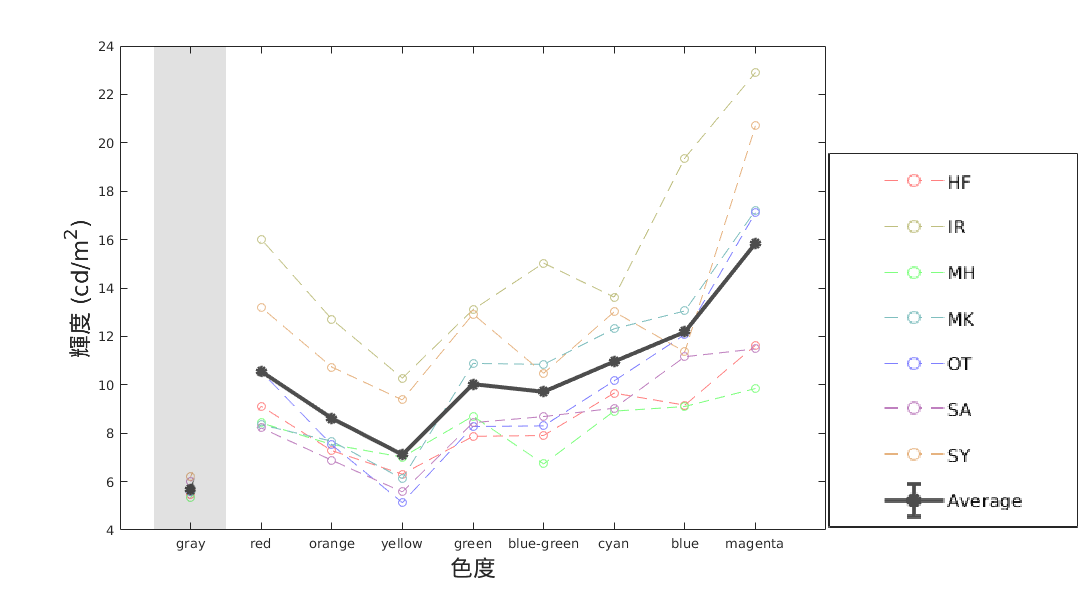
\includegraphics[width=14.0cm]{./img/ex2_res_SD_p.png}
                \caption{SD条件におけるテスト刺激の輝度}
                \label{ex2_SD}
            \end{figure}

            \begin{figure}[h]
                \centering
                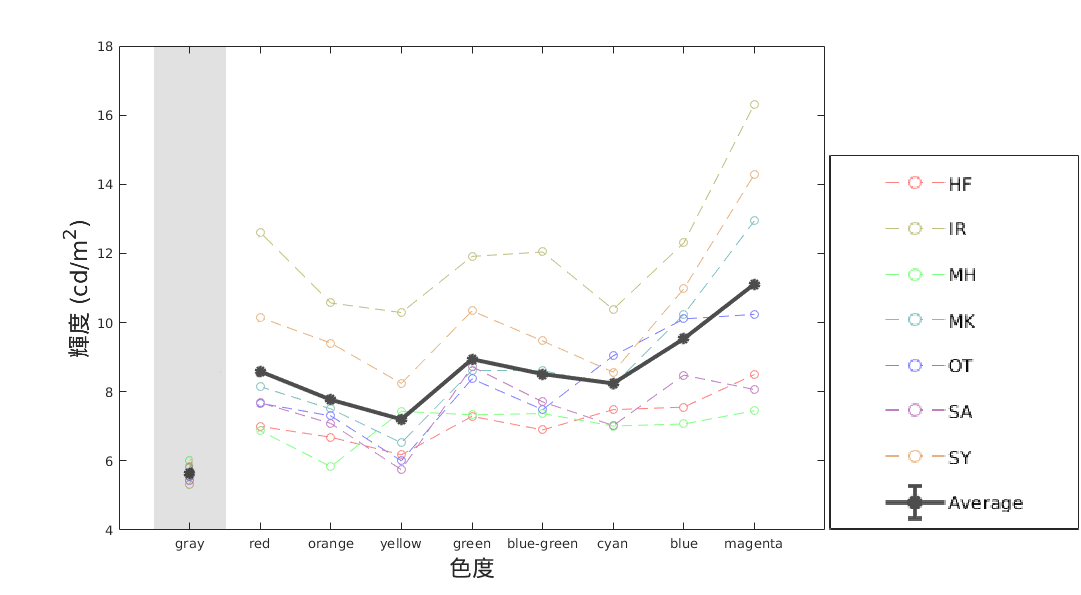
\includegraphics[width=14.0cm]{./img/ex2_res_D_p.png}
                \caption{D条件におけるテスト刺激の輝度}
                \label{ex2_D}
            \end{figure}

            図\ref{ex2_SD}がSD条件の結果,図\ref{ex2_D}がD条件の結果である.
            それぞれのグラフにおいて,横軸が刺激色,縦軸が被験者が調整したテスト刺激の輝度を示す.
            また,破線は被験者ごとの結果を表し,色が各被験者に対応している.
            黒実線は被験者間平均の結果を表す.
            どちらの条件においても,magentaの輝度が非常に高く,一方でgrayに次いでyellowの輝度が小さかった.

            個人差に着目しても,SD条件,D条件共に色度に対する応答の傾向に大きな違いは見られなかった.
            また,有彩色のテスト刺激の輝度値は,全体的にD条件よりSD条件の方が大きかったが,これは刺激彩度が大きかったことによりH-K効果も強く出たものと考えられる.

            本実験により,実験1で用いた刺激の平均色に対するHK効果を定量化できた.
            次節では,この結果と実験1の結果から,光沢感と明るさの関連性を検証する.

    \newpage
        \subsection{実験1との関連性}

            \begin{figure}[h]
                \centering
                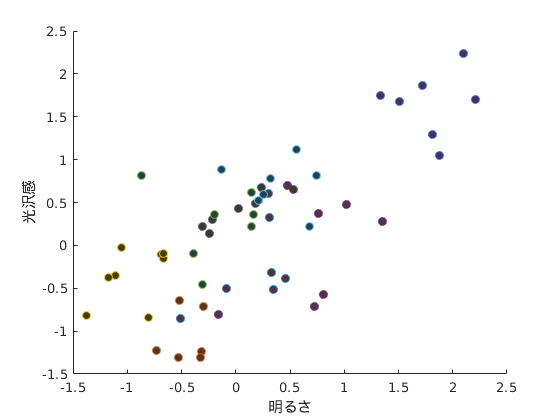
\includegraphics[width=11.0cm]{./img/ex3_DSD.png}
                \caption{Dragon形状のSD条件における散布図}
                \label{ex3_DSD}
            \end{figure}

            \begin{figure}[h]
                \centering
                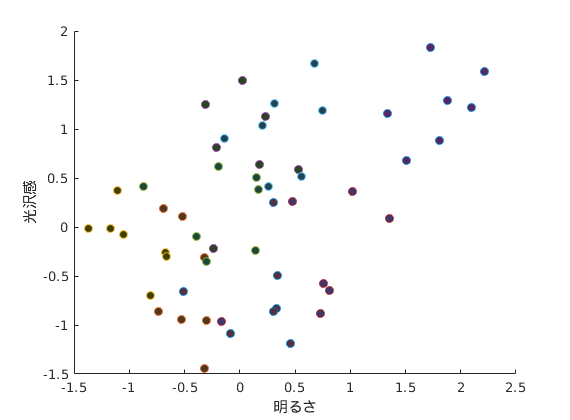
\includegraphics[width=11.0cm]{./img/ex3_BSD.png}
                \caption{Bunny形状のSD条件における散布図}
                \label{ex3_BSD}
            \end{figure}

            \newpage
            \begin{figure}[h]
                \centering
                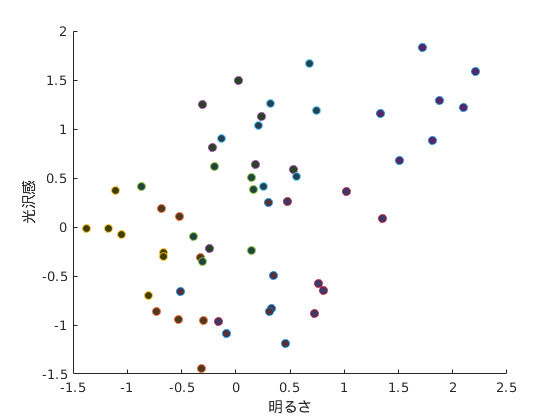
\includegraphics[width=11.0cm]{./img/ex3_DD.png}
                \caption{Dragon形状のD条件における散布図}
                \label{ex3_DD}
            \end{figure}

            \begin{figure}[h]
                \centering
                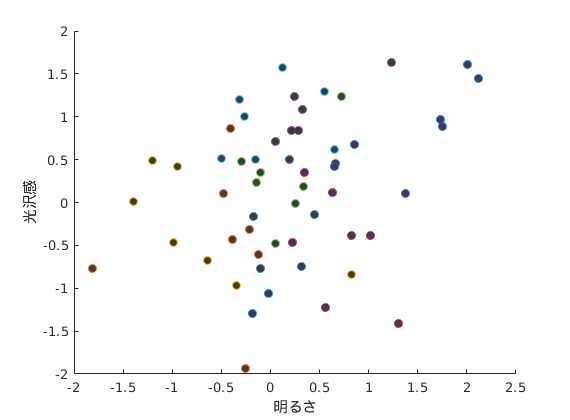
\includegraphics[width=11.0cm]{./img/ex3_BD.png}
                \caption{Bunny形状のD条件における散布図}
                \label{ex3_BD}
            \end{figure}

            \begin{table}[h]
                \centering
                \caption{各条件における実験1と実験2の結果の相関係数}
                \begin{tabular}{|l||c|c|} \hline
                                & SD       & D        \\ \hline \hline
                    Dragon      & 0.8828   & 0.8290   \\ \hline
                    Bunny       & 0.6490   & 0.5184   \\ \hline
                \end{tabular}
                \label{cc}
            \end{table}

            図\ref{ex3_DSD}から図\ref{ex3_BD}は,実験1と実験2のデータの両方に正規化を行い,物体形状と条件ごとに散布図にプロットしたものである.
            各点の色は実験で使われた9種類の色度からなり,横軸は明るさを,縦軸は光沢感を表す.
            また表\ref{cc}は各物体形状・着色条件における相関係数を表す.

            Dragon形状におけるSD条件,Dragon形状におけるD条件において比較的強い正の相関が見られたが,これに比べてBunny形状におけるSD条件,Bunny形状におけるD条件の相関係数は小さい値を示した.
            
            また,明るさ感と光沢感の相関を色度ごとに調べたところ,特にyellowでは明るさ感に対して光沢感の値が大きく,blueでは明るさ感に対して光沢感の値が小さかった.


        \subsection{考察}
        
            本実験の目的は,刺激全体の明るさ感が色度による光沢感増強効果を決定している可能性を検証することであった.
            実験結果では,いずれの形状・SD/D彩色条件に関わらず,光沢感と明るさに関して正の相関が得られた.
            これは,刺激全体から知覚される明るさが光沢感知覚に寄与していることが示唆された.

            一方で,明るさ感と光沢感の関係性が崩れている色相が存在した.
            この結果は,これらの色相においては光沢感変化は明るさ感からは予測できないことを示しており,これらの色相では明るさ感以外の要因が光沢感を変調したと考えられる.
            その要因の候補として,色度そのものが直接的に光沢感を変調させた可能性が考えられる.

    \newpage
\chapter{総合考察}
    \section{光沢感知覚に対する色度情報の寄与}
        本研究で行った実験から,色度情報が光沢感知覚に寄与することが示唆された.
        本研究の目的は,色度情報が光沢感に寄与するかどうか,また寄与する場合にはどのような要因が考えられるかを心理物理実験により明らかにすることであった.

        被験者にコンピュータグラフィックスとして生成された,輝度は同一であるが色度が異なる複数の画像刺激を呈示した.
        明るさ感のコントラストが光沢感に寄与しているという仮説をもとに,拡散反射成分と鏡面反射成分の両方に色度を付与するSD条件,拡散反射成分のみに色度を付与するD条件の2種類の条件を設定し,それらの条件をStanford DragonとStanford Bunnyの2種類の形状にそれぞれ適用した.
        被験者は,これらの刺激において,光沢感をより感じられる方を選択し,形状と条件間において色度ごとの光沢感を定量化した.

        この実験の結果,各形状と条件間で色度ごとの光沢感が異なることから,光沢感知覚に色度情報が寄与していることが示された.
        また,SD条件とD条件において応答の傾向に大きな違いが見られないことから,明るさ感のコントラストが光沢感に寄与しているという仮説が棄却された.
        加えて,刺激全体の明るさ感が光沢感に寄与している可能性が示唆された.

        次に,刺激全体の明るさ感が光沢感に寄与しているかを調べるために,上記の実験で用いた刺激の明るさ感を,刺激の平均色のパッチを用いることで測定した.
        さらに,測定された光沢感と明るさ感の関連性を調べることで,光沢感への明るさ感の寄与の度合いを算出した.

        この実験の結果では,Dragon形状のSD条件における明るさと光沢感の相関に強い正の相関があり,Bunny形状のD条件における明るさ感と光沢感の相関に比較的弱い正の相関があった.
        このことから,光沢感に明るさ感が寄与する可能性が高いが,それ以外の別の要因も光沢感に寄与している可能性が示唆された.


    \section{今後の課題}
        本研究では光沢感に明るさ感以外の要因が寄与している可能性が示唆されたが,具体的にそれがどのようなものであるかを明らかにすることはできなかった.


    \newpage
%\chapter{Conclusion}
\chapter{結論}

    本研究で得られた結論を以下に述べる.
    \begin{itemize}
        \item 輝度は同一であるが色度が異なるコンピュータグラフィックス画像間で光沢感を比較したところ,色度による有意な差が見られた.この結果から,光沢感知覚は輝度情報だけでは決定されず,色度情報も寄与していることが明らかになった.
        \item 拡散反射成分と鏡面反射成分の両方に色度を付与した刺激と拡散反射成分のみに色度を付与した刺激間で光沢感を比較したところ,色度による光沢感の傾向に大きな違いは見られなかった.もし鏡面反射成分と拡散反射成分の間の明るさコントラストが光沢感に寄与するのであれば,拡散反射成分のみに色度を付与した場合にはその明るさ感が増加することで鏡面/拡散反射成分間のコントラストが小さくなり,光沢感が減衰するはずであった.この結果から,光沢感に関して,鏡面反射成分と拡散反射成分の間の明るさ感コントラストの寄与は小さいことが示唆された.
        \item 刺激色度ごとに知覚される光沢感と明るさ感の関連性を調べたところ,それらに相関が見られたものの,黄色や紫色などにおいて明るさ感は小さいのに対して光沢感が顕著に高くなる傾向が見られた.この結果から,光沢感知覚に明るさ感も寄与している可能性が高いこと,ただし,刺激の色度も直接的に光沢感知覚に影響を与える可能性が示唆された.
    \end{itemize}
    \newpage
%\chapter*{Acknowledgements}
%\addchapter{Acknowledgements}
\chapter*{謝辞}
\addchapter{謝辞}

% 皆さんに感謝.皆さんに感謝.皆さんに感謝.皆さんに感謝.
% 皆さんに感謝.皆さんに感謝.皆さんに感謝.皆さんに感謝.
% 皆さんに感謝.皆さんに感謝.皆さんに感謝.皆さんに感謝.

%\addchapter{References}
\addchapter{参考文献}
\begin{thebibliography}{9}% 文献数が10未満の時 {9},10~99の時 {99}

\bibitem{Material}
    Fleming, R, W., Wiebel, C., Gegenfurtner, K. (2013).
    Perceptual qualities and material classes.
    {\it Journal of Vision}, 13(8):9, 1-20.

\bibitem{Motoyoshi}
    Motoyoshi, I., Nishida, S., Sharan, L., Adelson, E, H. (2007).
    Image statistics and the perception of surface qualities.
    {\it Nature}, 447, 206-209.

\bibitem{Marlow1}
    Marlow, P, J., Todorovic, D., Anderson, B, L. (2015).
    Coupled computations of three-deimensional shape and material.
    {\it Current Biology}, 25(6):16, 221-222.

\bibitem{Marlow2}
    Marlow, P, J., Kim, J., Anderson, B, L. (2012).
    The Perception and Misperception of Specular Surface Reflectance.
    {\it Current Biology}, 22(20):23, 1909-1913.

\bibitem{H-K effect}

\bibitem{Nishida}
    Nishida, S., Motoyoshi, I., Nakano, L., Li, Y., Sharan, L., Adelson, E, H. (2008).
    Do colored highlights look like highlights?
    {\it Journal of Vision}, 8(6):339.

\bibitem{Hunter}
    Hunter, R, S. (1937).
    Methods of determining gloss.
    {\it Journal of Research of the National Bureau of Standards}, 18.

\bibitem{Psychtoolbox}
    Brainard, D. H. (1997).
    The psychophysics toolbox.
    {\it Spatial Vision}, 10, 433-436.

\bibitem{Mitsuba}
    Mitsuba - physically based renderer. https://www.mitsuba-renderer.org/

\bibitem{StanfordModels}
    Turk, G., Levoy, M. (2005).
    Stanford University Computer Graphics Laboratory.

\bibitem{Ward}
    Ward, G. J. (1992).
    Measuring and Modeling anisotropic reflection.
    {\it Proceedings of the 19th SIG-GRAPH}, 265-272.



\end{thebibliography}

%\appendix
%\chapter{Proof of Theorem 1}\label{appendix1}
\chapter{定理1の証明}\label{appendix1}

%\chapter{Proof of Theorem 2}\label{appendix2}
\chapter{定理2の証明}\label{appendix2}

% ----------------------------------------------------------------------
\end{document}
